\chapter{Introduction}
  Particle physics aims to characterize the fundamental constituents of matter and the mechanisms by which they interact. The current state of the art theory is called \emph{The Standard Model of Particle Physics} (henceforth, just the standard model), which is written in the framework of \emph{Quantum Field Theory} (QFT).

  Though the standard model has been shown to make accurate predictions in a wide range of particle physics experiments, there are no shortage of open questions as to the origin of its structure. Furthermore, the standard model does not attempt to describe gravitation, and the observation of massive neutrinos prove definitively that the standard model must be incomplete. Another observation which strongly implies a deficiency is the evidence of at least one so-called \emph{dark matter} particle, an abundant particle which does not couple to the photon with any non-trivial strength. None-the-less, it is clear that the theory which supersedes the standard model must reduce to it in the appropriate limit, and its successes should not be downplayed.

  This thesis presents the search for a dark matter candidate which couples either directly or indirectly to the Z boson. The final states studied include multiple hadronic jets, transverse momentum imbalance, and a pair of opposite-charge same-flavor leptons having dilepton mass consistent with the pole mass of the Z boson. These final states are motivated by the strengths of the CMS detector as well as simplified models of supersymmetry, a systematic framework for extending the standard model. 

\section{The standard model of particle physics}
  Nearing the turn of the 20th century, the debate on the existence of elementary particles had still not been completely settled. But in the following 80 years, a wildly rich and successful theory of matter would be developed, culminating in what is called the standard model, which has been called the best tested theory in science.

  \subsection{The evolution of particle physics}
   J.J. Thomson is credited with finding the very first elementary particle, \cite{thomson_electron} the electron. Thomson observed that cathode rays, now known to be streams of electrons, would bend under the influence of a magnetic field. This implied that rays were a beam of particles, as opposed to some sort of aether phenomena, the competing theory at the time, because they responded in accordance with the known force law for charged particles. Thomson was able to deduce the charge to mass ratio for the electrons and found it was the largest charge-to-mass ratio ever measured for ionic gases, 3 orders of magnitude smaller than hydrogen ions.

   Thomson's student, Ernest Rutherford pushed the field of particle physics further when he discovered the nucleus, and later the proton. Rutherford famously shot alpha particles (hydrogen nuclei) at a thin sheet of gold. He found that the particles mostly passed through the sheets, which implied the gold was actually not a continuous material, but a lumpy collection of particles bound together. Einstein postulated the photon due to the photoelectric effect in the 1920s. The Neutron is discovered by James Chadwick in the 1930s after hearing about a series of experiments performed by German and French Physicists found that alpha particles striking beryllium would create a penetrating radiation that was not influenced by electric fields. 

   In the early 1930s Hideki Yukawa used the size of the atomic nucleus to predict the existence of pions, now known to be the carriers of the strong force which counteract the repulsion of protons in the nucleus due to their charge. When looking for pions, cosmic ray experiments found muons, and mistakingly believed they had confirmed Yukawa's theory. Muons were eventually shown to not interact much with nuclei, and so they were ruled out as nuclear force carriers. Pions are produced in large numbers in the upper atmosphere, but tend to disintegrate on their way to the ground. They were eventually discovered by comic ray experiments performed in the Andes mountains.

   During the same time period, Dirac predicted the existence of antiparticles using his mathematically correct, but philosophically misguided theory of holes. The positron was discovered by Anderson when he exposed a cloud chamber to a magnetic field and discovered electron/positron pair production. Another bit of elementary particle physics uncovered during this fruitful 1930s era was that of the existence of the neutrino, which was famously theorized by Wolfgang Pauli in order to salvage energy conservation in beta decay. Enrico Fermi unified Pauli's idea with the discovery of the neutron by hypothesizing that beta decay was the decay of a neutron into a proton, an electron, and a neutrino. The electron anti-neutrino was finally discovered by observing reverse beta capture. Further observations showed muons could decay to electrons, but only in association with two neutrinos. This lead to the notion that neutrinos must carry "lepton flavor," in other words, there must be a neutrino for each lepton.

   By the 1950s, particle accelerators began to appear, and so too did the observation of a ``zoo" of new particles. These particles included some mesons which had a \emph{strangely} long lifetime, like the K$^0$, and a slew of other heavy particles. Observations suggested strange particle were always produced with another strange partner, but there was no such restriction on their decays. That fact, in addition to the long lifetime of strange particles hinted that their decays were mediated by a different force than their creation. This lead to the notion of conservation of strangeness whereby each particle was assigned a strangeness of 1, 0, or -1. Along with conservation of baryon number (theorized by Stückelberg to stabilize the proton), conservation of lepton number, and conservation of charge, a series of discrete symmetries began to appear for elementary particles. 

   Using charge and strangeness values for particles, Murray Gell-Mann developed the famous ``eightfold way," a scheme for laying out particles in geometrical patterns based on their charge and strangeness values. Arranging the particles in this way inferred the existence of a heavy particle with negative charge and -3 strangeness, now called the $\Omega^-$, which had not been observed. The observation of the $\Omega^-$ ushered in an era of particle physics which was based on symmetry principles, a trend which still dominates the field to this day.

  \begin{figure}[h!]
    \begin{picture}(150, 150)(-100, -30)
      \put(-25,42){\line(-3,-5){25}}
      \put(-25, 42){\line(1, 0){50}}
      \put(25, 42){\line(3,-5){25}}
      \put(-25, -42){\line(1,0){50}}
      \put(-25, -42){\line(-3, 5){25}}
      \put(25, -42){\line(3, 5){25}}

      \put(-25, 42){\circle*{3}}
      \put(-25, -42){\circle*{3}}
      \put(25, 42){\circle*{3}}
      \put(25, -42){\circle*{3}}
      \put(-50, 0){\circle*{3}}

      \put(50, 0){\circle*{3}}
      \put(0, 3){\circle*{3}}
      \put(0, -3){\circle*{3}}

      \put(-28, 47){$K^{0}$}
      \put(28, 47){$K^{+}$}
      \put(-28, -55){$K^{-}$}
      \put(28, -55){$\overline{K}^{0}$}
      \put(55, 0){$\pi^{+}$}
      \put(-65, 0){$\pi^{-}$}
      \put(0, 10){$\pi^{0}$}
      \put(0, -15){$\eta$}

      \put(-120, 43){$s=1$}
      \put(-120, 0){$s=0$}
      \put(-120, -43){$s=-1$}

      \put(-20, -85){$q=-1$}
      \put(45, -85){$q=0$}
      \put(70, -30){$q=1$}
    \end{picture}

    \begin{picture}(150, 150)(-375, -200)
      \put(-75,42){\line(3,-5){75}}
      \put(-75, 42){\line(1, 0){150}}
      \put(75, 42){\line(-3,-5){75}}

      \put(-25, 42){\circle*{3}}
      \put(-25, -42){\circle*{3}}
      \put(25, 42){\circle*{3}}
      \put(25, -42){\circle*{3}}
      \put(-50, 0){\circle*{3}}
      \put(50, 0){\circle*{3}}
      \put(0, 0){\circle*{3}}
      \put(0, -84){\circle*{3}}
      \put(-75, 42){\circle*{3}}
      \put(75, 42){\circle*{3}}

      \put(-78, 47){$\Delta^{-}$}
      \put(-28, 47){$\Delta^{0}$}
      \put(28, 47){$\Delta^{+}$}
      \put(78, 47){$\Delta^{++}$}
      \put(-20, -45){$\Xi^{*-}$}
      \put(30, -45){$\Xi^{*0}$}
      \put(55, 0){$\Sigma ^{*+}$}
      \put(-45, 0){$\Sigma^{*-}$}
      \put(5, 0){$\Sigma^{*0}$}
      \put(5, -84){$\Omega^{-}$}

      \put(-120, 43){$s=0$}
      \put(-120, 0){$s=-1$}
      \put(-120, -43){$s=-2$}
      \put(-120, -85){$s=-3$}

      \put(10, -120){$q=-1$}
      \put(42, -75){$q=0$}
      \put(75, -25){$q=1$}
      \put(105, 15){$q=2$}
    \end{picture}
    \vspace*{-50pt}
    \caption{The meson octet (left) and the baryon decuplet (right). Murray Gell-Mann arrayed elementary particles in these patterns and used them to predict the existence of the $\Omega^-$. This sparked a revolution in elementary particle physics based on discrete symmetries. \cite{eightfold_way}}
  \end{figure}

    Gell-Mann and Zweig independently proposed that the origin of these patterns were due to the fact that hadrons are made up of \emph{quarks}. The quark model was successful at reproducing the predictions of the eightfold way, and gave a mechanism for why particles with certain electric charges, masses, and decay pathways exist while others don't. Additionally, deep inelastic scattering experiments, much the same as Rutherford's, showed that the charge inside protons also seem to be collected in lumps, and in a way that is consistent with the three fractionally charged partons described in the quark model. \cite{proton_structure} The quark model eventually became encoded in Quantum Chromodynamics, which took it's modern form in the early 1970s with the discovery of assymptotic freedom.

    In the 1930s, the theoretical problem of infinities in quantum field theory began to emerge, specifically when calculating the mass of the electron. By the 1950s, much of the theoretical foundation for Quantum Field Theory had been laid in pursuit of a theory of Quantum Electrodynmanics (QED). Julian Schwinger and Sin-itiro Tomonaga independently developed a formalism based on operator mathematics. This approach was shown to be equivalent to a formalism developed by Richard Feynman using path integrals by Freeman Dyson in 1949.\footnote{The prominant physicist Oppenheimer was so sure that Feynman's ideas were wrong that Dyson's proof earned him a lifetime appointment at the Institute for Advanced Study in Princeton without ever needing to earn a PhD.} The theoretical progress during this time explained the observation of the Lamb shift in the spectrum of hydrogen, and the electron's anomalous magnetic moment, a computation which is experimentally verified to better than 1 part per billion and has elevated the standard model to be called the best tested theory in science. In formulating the equivalence of theories, Dyson laid out criteria to decide whether a theory was renormalizable, an important feature expected from any physical QFT.

    In the 1950s an enormous theoretical breakthrough was made by Yang and Mills, who developed the concept of a Gauge theory. The gauge group SU(2)xU(1) was found to be at the heart of the unified theory of the electromagnetic and weak interactions, now called electroweak theory. Steven Weinberg invoked the Higgs mechanism in 1967 to bring the theory into modern form, showing that a massless theory in the high energy limit could "spontaneous break" into a theory with a massless photon but massive Ws and Zs at laboratory energy scales. Weinberg's theory required the existence of a scalar boson called the Higgs. \cite{Weinberg_EWK} His theory was partially confirmed with the discovery of the W and Z bosons at the UA1 and UA2 experiments at CERN in 1973. The final prediction of the electroweak theory was verified in 2012 with the discovery Higgs boson decaying to 2 photons in 2012 by the CMS and ATLAS collaborations at the Large Hadron Collider. \cite{CMS_higgs,ATLAS_higgs} The search presented in this thesis was conducted within the CMS collaboration.

    With the combination of QCD and electroweak theory, a total Lagrangian could be written with the symmetry group SU(3)xSU(2)xU(1), this is now what we called the standard model. But the particle content of the standard model still was being discovered into the next decade. In the 1970s, several breakthroughs were made. The discovery of the J/Psi meson in 1974 confirmed the existence of a fourth heavier quark, now called the charm. This brought the total number of known quarks to 4. However in the previous year experiments showed violation of CP symmetry in Kaon decays, and it was worked out by Kobayashi and Maskawa that a 4 quark model could not accommodate CP violation, at least 6 quarks were needed. 

    In 1975, the Tau lepton and it's neutrino were discovered, which gave another hint that there were 6 quarks, as it seemed natural to have the same number of quarks and leptons. Finally 1977, the bottom quark was discovered at Fermilab, giving further evidence of a sixth quark. The final piece of the puzzle was the detection of the top quark in 1995 in proton-antiproton collisions at Fermilab.


    As described above, the standard model has successfully predicted the existence of the W, Z, and Higgs bosons, including their decays. It predicted the electrons anomalous magnetic moment to extremely high precisions. It predicted the existence of a third generation of quarks and leptons based on CP violation. Indeed, at the current state of affairs, the standard model it incorporates essentially all known particle phenomenology except neutrino masses and dark matter.

  \subsection{The framework of Quantum Field Theory}
    Quantum Field Theory is the framework of the standard model. A ``theory" in particle physics typically refers to a function on spacetime called the \emph{Lagrangian Density} or simply the Lagrangian. The Lagrangian which describes the interaction of charged particles with electromagnetic fields, the function that defines quantum electrodynamics (QED), can be written 

    \[
      \mathcal{L} = i \bar\psi \gamma^\mu \partial_\mu \psi - e\bar{\psi}\gamma_\mu (A^\mu+B^\mu) \psi -m \bar{\psi} \psi - \frac{1}{4}F_{\mu\nu}F^{\mu\nu}.
    \]

    The symbols $\psi, A, B,$ and $F$ represent fields, which means they are functions that associate a tensor\footnote{roughly a matrix, which includes objects like vectors and numbers} to each point in spacetime. In very rough terms, when the value of the tensor at some point in spacetime is nonzero, that represents the presence of a particle at that point. Any term in the sum where two fields are multiplied is called a coupling between fields, and it represents that energy can flow directly between the two fields.

    The first term, called the ``kinetic term", represents the fact that particle motion takes energy, it couples the derivative of, or change in, $\psi$ to the value of $\psi$. The second term represents the coupling of the electric and magnetic fields with the charged particle, the constant $e$ represents an elementary charge (like the charge of the electron), and it regulates the strength of the coupling. The third term, the coupling of $\psi$ with itself, represents the mass of the charged particle, with $m$ being the strength at which $\psi$ couples to itself. The final term represents that energy can flow between the electric and magnetic fields.

    One of the many beautiful aspects of the Lagrangian formalism is the additivity of theories. The above describes electromagnetism, 

    Lagrangians and Feynman rules, show the S.M. Lagrangian, explain terms. Particles are fields, etc...
\section{Problems with the Standard Model} \label{sec:problems_with_sm}
  Though the standard model has had incredible successes, there are still many open questions:
  \begin{enumerate}
    \item Observations in astronomy show that particle content based on the standard model can not explain the galactic rotation curves.
    \item Why are there three generations?
    \item There is precedent to assume that at high enough energies, all three forces in the standard model combine into a single grand unified theory (GUT). The energy at which this occurs is typically called the GUT scale. Using the methods of renormalization, one can fine the GUT scale to be between $10^15$ and $10^16$ GeV. It is a mystery as to why this scale is so different from the electroweak scale (the mass of the Higgs boson).
    \item
  \end{enumerate}
  
  \subsection{Dark Matter and Dark Energy: The Tension with Astrophysics}
      Dark matter, dark energy, neutrino masses, gravitation, inflation
      Curiosities: Why 3 generations, should there be naturalness, unstable universe
      Deviations: TTH xsec, muon magnetic moment, Lep forward backward b-bbar asymmetry.
      Leptons in this document refer to light leptons, electrons or muons.
  \subsection{The Solutions of Supersymmetry}
    Supersymmetry (SUSY) is a framework which can be used to build infinitely many extensions of the SM. The key idea behind SUSY is the treatment of boson and fermion fields as pairs, called \emph{superpartners}.\footnote{The most commonly cited review is \cite{susy_primer}} A Lagrangian is called supersymmetric, roughly, if you can interchange the two superpartners without changing its physical predictions. It illustrates the right flavor to say ``the superpartners experience the same interactions."\footnote{This is an overstatement. In reality, supersymmetry transformation are built on infinitesimal translations of the fields. Fields and their superpartners will be mathematical objects with different dimensions, a strict substitution doesn't truly make sense. \todo{Is this right?}}

    SUSY can be traced back to the late 1960s, with the first physical models of SUSY in 4 dimensions discovered by Weiss and Zumio in the 1974. \cite[ch. 24]{weinberg_SUSY} There are many reasons why physicists like SUSY, a few are listed below

    \begin{itemize}
    \item Mathematically, supersymmetry is the only known caveat to the Coleman-Mandula theorem, which states that the symmetry group of non-trivial QFTs must be written as
      \[
      G_{\text{Poincaré}} \times G_{\text{internal}}.
      \]
      This result is known as the Haag–Łopuszański–Sohnius theorem. Broadly speaking, supersymmetry is the only known caveat to a quite strong restriction on the structure of QFTs.
    \item Supersymmetry offers a solution to the naturalness problem described in section \ref{sec:problems_with_sm} by automatically including exactly canceling counter-terms for the large quantum corrections to scalar particle masses, like the Higgs mass.
    \item In models with R-parity conservation, described below, supersymmetry provides a natural dark matter candidate. The lightest supersymmetric particle (LSP) should not be able to decay to regular matter because of the conservation law, and so an electrically neutral LSP could be the dark matter we see in astrophysical observations.
    \item The minimal supersymmetric extension to the standard model, i.e. the addition of one superpartner for each SM particle, seems to be able to accomodate predicts that the
    \end{itemize}

    \begin{figure}[h!]
    \centering
    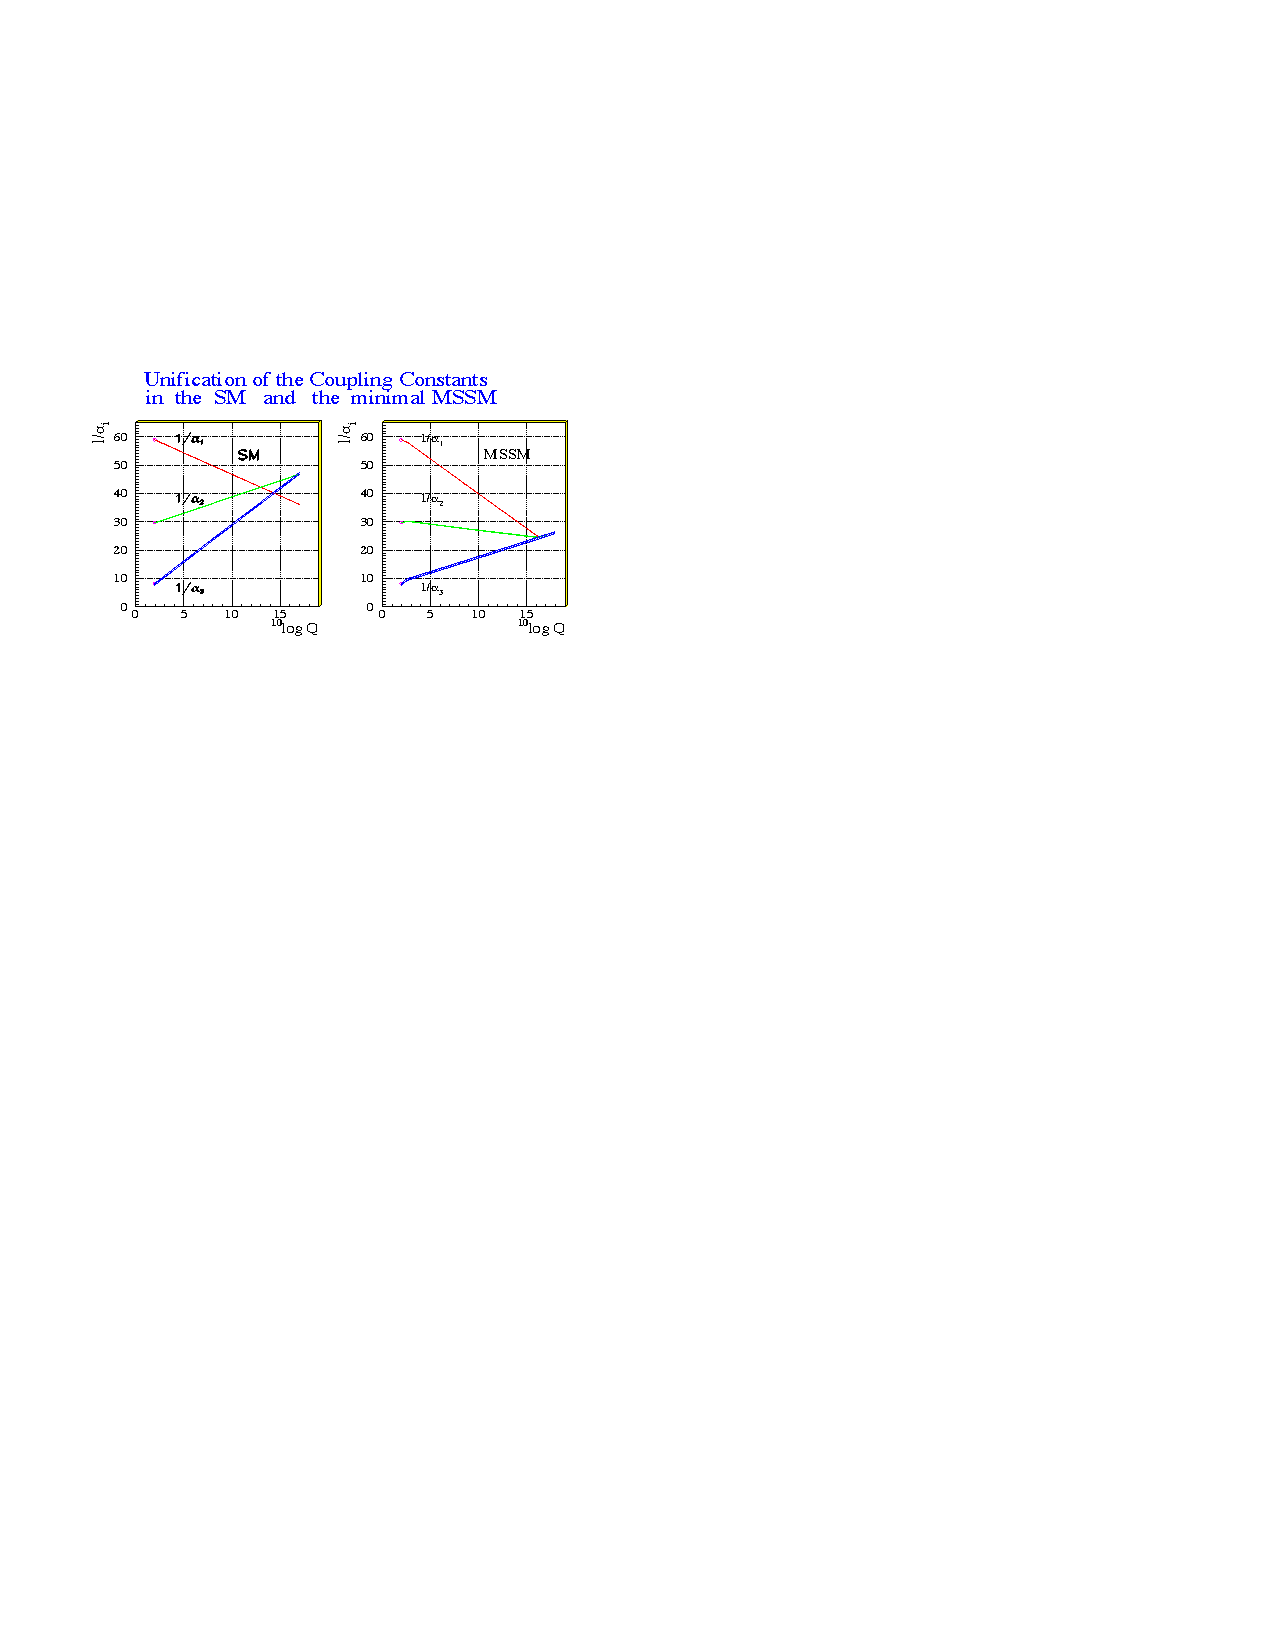
\includegraphics[width=.7\textwidth]{figures/SUSY_GUT_couplings.pdf}
    \caption{The strength of the strong[SU(3)] and electroweak [SU(2)xU(1)] coupling constants. On the left, the prediction derived from the standard model is shown, and the right the predictions from the MSSM. In a grand unified theory, the lines are expected to meet at a single point where all the forces unite and therefore have equal strength. There are 8 standard deviations separating a perfect fit for the standard model (i.e. assuming no new particles heavier than the top quark exist), while the MSSM accommodates a unification point much more readily. This is interpreted as a sign that the MSSM might be the legitimate GUT of nature. Taken from \cite{SUSY_RG}}
    \label{fig:susy_gut}
    \end{figure}

     It is mathematically interesting because supersymmetric QFTs are much easier to analyze theoretically, and because supersymmetry transformations are the only known caveat to the Coleman-Mandula theorem which states that the symmetry group of a non-trivial\footnote{i.e. one in which particles can interact} QFT must take the form 

    \[
      G_{\text{Poincaré}} \times G_{\text{internal}}.
    \]

     so that for every fermion field, there is a boson field such that the Lagrangian would be identical if the interactions of the boson field were replaced, in a special way, by the fermion field and visa versa. treats matter and forces as pairs. It keeps the higgs mass a natural parameter. Grand unification becomes possible. LSP is a dark matter candidate in R-parity preserving theories.
      Wiess and Zumio
      GUT miracle, coleman-mandula, naturalness

      coleman mandula states that symmetry groups in QFTs must be of the form Poincare x Internal. Haag–Łopuszański–Sohnius theorem shows that it can also be supersymmetry, i.e. when conserved quantities are spinors (higher fermionic stuff ruled out mathematically). So basically you have an interesting mathematical result, why are these symmetries allowed which break a common no-go-theorem?
    \subsubsection{R-parity} \label{sec:r-parity}
      Proton lifetime, dark matter candidate
    \subsubsection{Simplified Models}
      What's the idea, MSSM, pMSSM, SMS (using only one new particle).
      GMSB: https://arxiv.org/pdf/hep-ph/9707450.pdf, https://arxiv.org/pdf/hep-ph/9801271.pdf
    \subsubsection{Parameter space}
      Not all susy needs to be at EWK scale, why do we think it should be? What can we actually rule out with these models?
\section{Why focus on the Z with \MET final state?}
  As mentioned in the introduction, the ZMET final state is motivated partially by considerations about the detector and partially by simplified supersymmetric models. Leptons at the LHC are rarely produced compared to hadronic jets,\ref{sec:what_gets_made} and are typically measured with high energy resolution (\ref{sec:electron_measurement_pipeline}, \ref{sec:muon_measurement_pipeline}). This makes a leptonically decaying Z boson a great object to tag as the energy resolution of the Z will be good and the standard model backgrounds for opposite-charge same-flavor leptons with dilepton mass near the Z pole mass is extremely low. The main production method of Z bosons in proton-proton collisions is Drell-Yan production. To reduce this background, we require at least 2 jets are 

  \subsection{Past results}
  An analysis in this final state has been published several times from the CMS collaboration, with the latest iteration in 2016.\cite{paper_2012, paper_2015, paper_2016} The differences between the previous version and the analysis presented in this thesis are summarized below:
  \begin{itemize}
    \item The integrated luminosity analyzed increased by a factor of 15.
    \item Search regions were added to target SUSY production leading to final states contain an additional W or Z boson (VZ), and final states containing a Higgs boson (HZ). Interpretations in simplified models that produce these final states were also added. \ref{sec:search_regions}
    \item A correction is now applied to the photon sample used in the Z+Hadronic background prediction to subtract away events with real \MET. \ref{sec:ewk_subtraction}
    \item A new method for the flavor symmetric background prediction was developed which uses same-sign events outside the Z mass window to predict the MET spectrum inside. \ref{sec:kappa}
  \end{itemize}